
\chapter*{L'Optimisation du Code}
\section*{La division}

L'opération la plus lognue dans notre kernel est la division. A chaque exécution du kernel, celle-ci est éxécutée $n^2$ fois.

On inverse les boucles, ainsi on ne fait plus que $n$ divisions ; mais on doit faire en plus $n^2$ multiplications par appel du kernel.
\\Sur les processeurs Ivy Bridge, la multiplication est environ 3$\times$ plus rapide que la divsion. En considérant qu'une multiplication est faite en 1 cycle, on peut donc comparer.
Sans les boucles inversées,le traitement fait $n^2$ divsions, pour une durée de $3n^2$.
Avec les boucles inversées,le traitement fait $n$ divisions et $n^2$ multiplications, soit une durée de $3n+n^2$.
On compare $3n^2$ et $3n+n^2$:\\
\begin{figure}[ht!]
    \centering
    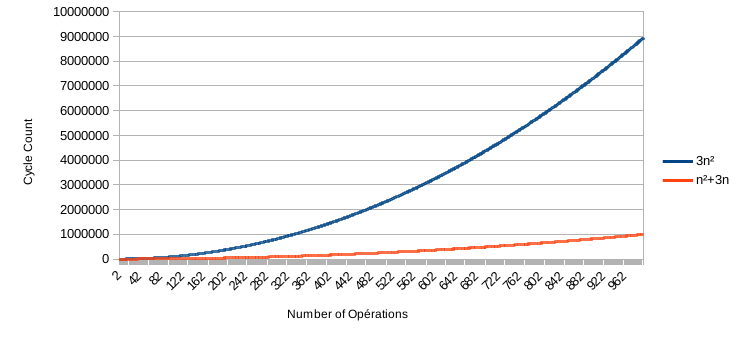
\includegraphics[width=100mm]{MEDIA/div_vs_mult_graph.png}
    \caption{Comparaison des temps de calcul des deux méthodes}
\end{figure}
Inverser les boucles est donc beaucoup plus rentable.
Speedup offert par cette optimisation:<A Calculer>

\section*{L'accès Indirect}

Une opération qui fait également perdre du temps au kernel est l'accés indirect sur le tableau a.
Nous proposons d'ajouter une boucle au début du noyeau qui calculera les accés indrects avant que ceux-ci soient utilisés dans la bocule de calcul.
Ces données doivent être stockées entre le temps, la première idée serait d'ajouter un tableau supplémentaire a cet effet, mais il faudrait alors recalculer toutes les tailles de tableau pour le L1, L2, L3 et RAM (n valeurs supplémentaires a stocker).\\

Pour ne pas consommer plus de mémoire, nous avons donc décidé de stocker ces valeurs sur la dernière ligne du tableau résultat.
Lors du calcul de la dernière ligne, l'indice indirect est donc lu pour la dernière fois juste avant d'être remplacé par le résultat. 

Speedup offert par cette optimisation:<A Calculer>


